\section{Ermittlung der konvexen Hülle}

Als eine konvexe Hülle wird eine Teilmenge einer euklidischen Gesamtmenge an Punkten bezeichnet, für die folgende Bedingung gilt: Wählt man aus der Gesamtmenge zwei beliebige Punkte, so ist die Strecke zwischen Ihnen immer komplett zwischen den Punkten der konvexen Hülle. Für die Bestimmen der konvexen Hülle von Punkten \(P\) in \( \mathbb{R}^2\) existieren verschiedenste Algorithmen, wie zum Beispiel der Monotone Chain von \citet{andrew1979another}, QuickHull nach \citet{eddy1977new} oder den Divide-and-Conquer Algorithmus von \citet{preparata1985convex}. Da alle diese Algorithmen ein ähnliches Laufzeitverhalten aufweisen, wird für die spätere Anwendung hier exemplarisch der Graham Scan nach \citet{graham1972efficient} näher erläutert. Dies ist einer der populärsten Algorithmen für die Berechnung der konvexen Hülle und besitzt eine Komplexität von \(O(n \log n)\).\\

Gestartet wird der Algorithmus mit der Menge aller Punkte \(P\) der Ebene und mit einem Startpunkt \(P_0\), der Bestandteil der konvexen Hülle ist. Hierzu wird meist der Punkt mit dem niedrigsten \(y\) Faktor gewählt. (\(P_0=P_{min(y)}\)) Listing \ref{lst:graham-scan} zeigt den Verlauf des Algorithmus des Graham Scans. Dabei wird in Abbildung \ref{fig:convexhull} nochmals die erste Sortierung und das Unterscheidungskriterium für die Sortierung als auch für die Aussortierung der Punkte verdeutlicht. \citep{convexHull} \\


\begin{lstlisting}[mathescape,caption=Graham Scan Algorithmus, label=lst:graham-scan, float=htbp]
Eingabe: Menge der Punkte $P$, außen liegender Punkt $P_0$
Ausgabe: Punkte der konvexen Hülle

$i$ = 0
sortiere nach dem Winkel zu $P_0$
solange $i$ <= $|P|$
    wenn $\measuredangle P_{i-1} P_{i}$ > $\measuredangle P_{i-1} P_{i+1}$, also $P_i$ rechts von  $\vec{P_{i-1} P_{i+1}}$ liegt
        inkrementiere $i$
    ansonsten
        entferne $P_i$ aus $P$
        dekrementiere $i$
    
\end{lstlisting} 

\begin{figure}[h]
  \centering
	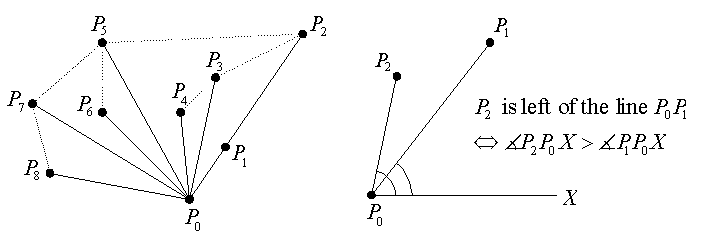
\includegraphics[width=0.9\textwidth]{content/images/methods/convexhull.png} 
  \caption{Sortierung der Punkte nach Winkel zum Startpunkt (links) mit dem Unterscheidungskriterium (rechts). Übernommen von \citet{convexHull}}
  \label{fig:convexhull}
\end{figure}
